{\em Auteurs: Arne Vlietinck \& Bram Vandendriessche}
\\\\
In deze sectie worden de resultaten die behaald zijn bij de verschillende onderdelen van het project, kort besproken. 
\subsection{Testbed}
Het Testbed voldoet aan alle vereisten die door de opgave zijn opgesteld. De simulator is in staat om een Polyhedron weer te geven in een 3D-wereld. Omwille van het ontwerp is het eenvoudig om nieuwe polyhedra aan te maken en toe te voegen aan de wereld. De generator kan een bestand te produceren dat volgens het opgegeven \textit{World description file format} een opstelling beschrijft. De \textit{parser} leest dit bestand in en stelt de beschreven 3D-wereld op. Objecten in de omgeving kunnen met behulp van de \textit{editor} worden toegevoegd, verplaatst en verwijderd.
\\
\noindent
Zoals reeds eerder vermeld is het met de finale implementatie van het Testbed moeilijk om onafhankelijke testen uit te voeren zonder een hele wereld te moeten voorzien. Dit is geen probleem indien een grote TestSuite moet worden uitgevoerd, maar erg nadelig voor het testen van individuele methodes, zoals bijvoorbeeld collision detection. Het zou daarom beter zijn indien het Testbed met verschillende lagen zou zijn ge\"implementeerd zodat de interne representatie kan bestaan zonder dat hier de grafische component van \textit{OpenGL} bij vereist is. Een ontkoppeling tussen de \textit{World} en \textit{WorldObjects} enerzijds en \textit{OpenGL} anderzijds zou dus een sterke verbetering zijn. Dit inzicht kwam er echter pas na het vak \textit{Software-Ontwerp}, waardoor er niet genoeg tijd was om het Testbed helemaal om te gooien. Deze conclusies werden wel toegepast op de 3D-component van de Autopilot.\\
\\
\noindent
Afgezien hiervan is het ontwerp wel goed in die zin dat nieuwe objecten (zowel drones als nieuwe figuren), makkelijk kunnen worden toegevoegd door ze te laten overerven van \textit{WorldObject}. Dit is een grote troef gebleken bij de toevoeging van polyhedra.


\subsection{Autopilot}
\subsubsection{Vliegen}
Bij de ontwikkeling van de Autopilot is er voor een opbouwende aanpak geopteerd. Dit wordt duidelijk in de verschillende voltooide functionaliteiten. Hierdoor is er een Autopilot beschikbaar met een gereduceerd aantal voltooide mijlpalen.\\
De drone is in staat om naar verschillende opeenvolgende punten te vliegen en hierbij de obstakels te ontwijken. Een grote hindernis die hier ondervonden werd, is de interpretatie van de rotaties. Deze zijn uitgewerkt zoals beschreven in Sectie \ref{sec: Rotaties}. Hier blijkt dat het voorziene testbed toch een andere interpretatie van de rotaties aanneemt, waardoor de Autopilot niet werkt op het voorziene Testbed.\\
Verschillende polyhedra kunnen doorprikt worden met ontwijken van de obstakels. Dit is een uitbreiding op het vorig puntje, aangezien de punten nu vervangen zijn door het herkennen en lokaliseren van polyhedra. \\
De windimplementatie werkt niet optimaal. De oorzaak van de fout is een niet correcte voorspelling van de snelheid. Daar de volgende snelheid gebaseerd is op de vorige snelheid wordt deze fout steeds groter en groter. Dit resulteert in een opbouwende fout tijdens de berekening van de compensatiekracht, waardoor de wind verkeerd wordt gecompenseerd. 

\subsubsection{Scannen}
Het scannen is beperkt gebleven tot slechts \'e\'en object, waarbij de simulator zorgt voor de beweging. De vliegstrategie hiervoor is uitgewerkt, maar werd niet toegepast omdat het erg lang heeft geduurd tot de drone in staat was om enigszins stabiel te vliegen. De Autopilot is dus ook niet in staat om de drone naar verschillende objecten te sturen en deze stuk voor stuk te scannen. \\
\\
\noindent
De kwaliteit van de scan is vrij tot zeer goed, afhankelijk van de moeilijkheidsgraad van het object, doordat punten constant gecorrigeerd en gematcht worden voor een mooi gesloten figuur. Bij vlakken die niet goed zichtbaar zijn (bv. bij de holle kubus), is de gescande figuur niet volledig correct aan de binnenkant. Deze figuur zou als niet-scanbaar moeten herkend worden. Deze error melding zit echter niet in de functionaliteiten van de drone omdat het door enige onzekerheid ook om een slecht gescande zichtbare figuur zou kunnen gaan.
\begin{figure}[H]
\centering
	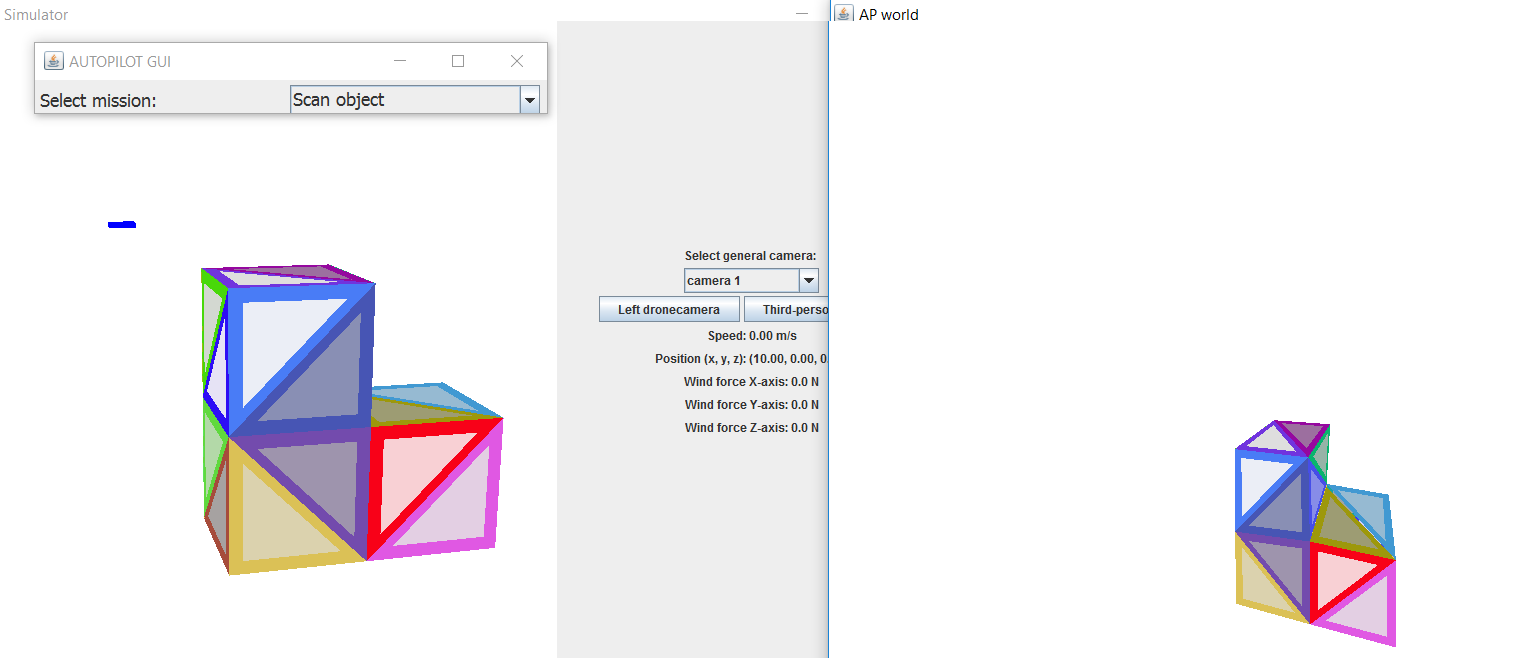
\includegraphics[width=0.6\textwidth]{letterL.png}
	\caption{Scan van een eenvoudige figuur.}
    \label{fig:ScanFly}
\end{figure}


\subsubsection{Wireprotocol}
De Autopilot is in staat om met een ander Testbed te verbinden door middel van het Wireprotocol. De implementatie hiervan staat in de klasse \textit{ConnectionProvTes}-klasse. Omwille van een verschillende interpretatie van assen en rotaties, reageert de drone echter niet zoals verwacht in het gegeven Testbed.